\chapter{Additional Experiments}\label{sec:appendix:add_exp}
In this first appendix, we describe some of the experiments that were conducted during the three year of thesis, but that were not included in the main part of thesis for diverse reasons. 

\section{Acquisition of Real-World Data}

\subsection{For Optical Flow}
Before making use of the \acrfull{fwl} metric in order to evaluate the quality of our optical flow results on high-resolution data, we initially tried to find an event-based dataset with a high-resolution camera and with a ground truth for optical flow. This research being unsuccessful, we decided to record our own dataset.

To do so, as illustrated in \cref{fig:appendix:add_exp:of_dataset_setup}, we used a Parrot Jumping Sumo minidrone as a moving object, and placed our event cameras (Prophesee Gen4~\cite{Finateu2020510A1} and DAVIS240C~\cite{Brandli2014A2}) directly above it, looking downwards. In order to generate the ground truth, we also added a high-resolution RGB camera (Allied Vision Mako G-192C) between the two event cameras, also looking downwards. Since the robot was evolving on the ground, and since its height was negligible compared to the height at which the cameras were positioned, an approximation of the robot moving on the ground being equivalent to a flat shape moving on a plane could be made. With this approximation, and with adequate calibration and synchronization between the cameras, a simple homography could then be applied to superimpose data from various cameras, as shown in \cref{fig:appendix:add_exp:of_superimposition}. Finally, by using a state-of-the-art optical flow method on the frames (RAFT~\cite{Teed2020RAFTRA}), and by applying our optical flow method on the events, a quantitative and qualitative comparison could then be made.

\begin{figure}
  \centering
  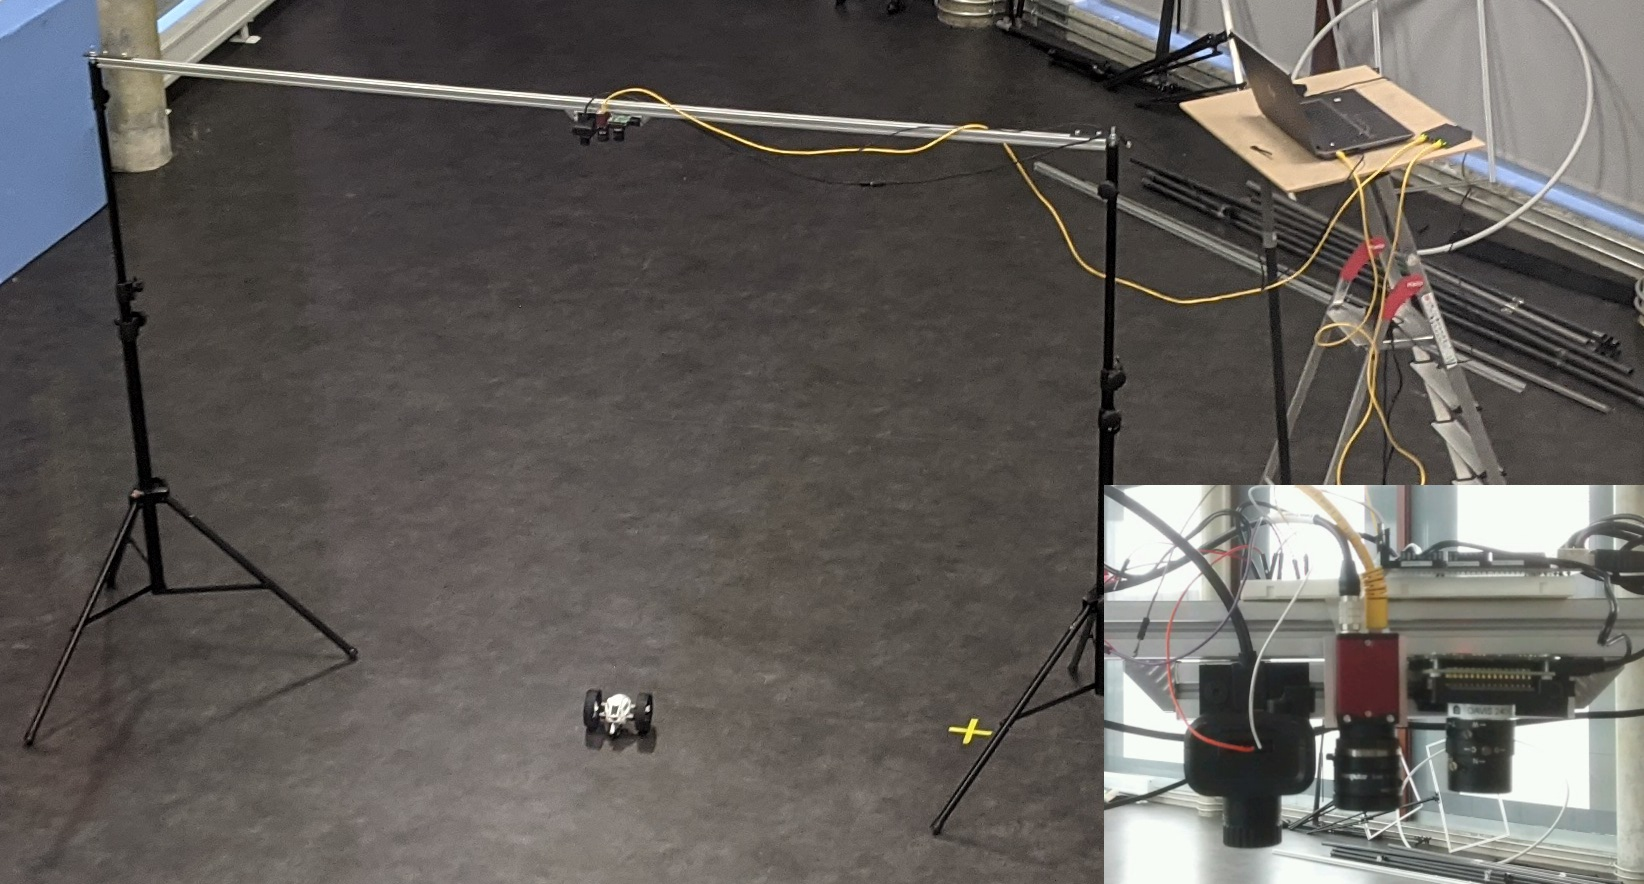
\includegraphics[width=0.85\linewidth]{mainmatter/figures/a_additional_exp/of_dataset/setup.jpg}
  \caption{Setup used for the recording of the optical flow dataset. The Parrot Jumping Sumo minidrone is visible in the center, and a zoomed view of the cameras (Prophesee Gen4 / Allied Vision Mako G-192C / DAVIS240C) is given at the bottom right.}\label{fig:appendix:add_exp:of_dataset_setup}
\end{figure}

\begin{figure}
  \centering
  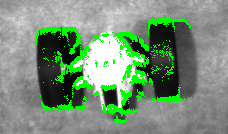
\includegraphics[width=0.3\linewidth]{mainmatter/figures/a_additional_exp/of_dataset/superimposed.png}
  \caption{Superimposed frame from the Mako camera (in grayscale) and events from the Prophesee camera (in green).}\label{fig:appendix:add_exp:of_superimposition}
\end{figure}

Five sequences were recorded, where the robot was following various patterns under the cameras: moving in a straight line, slaloming, drawing a circle, drawing a square, and moving in a straight line with a second robot coming from the opposite direction. An example of results is shown in \cref{fig:appendix:add_exp:of_results}, and a playlist of videos is available at {\small\url{https://www.youtube.com/playlist?list=PLLL0eWAd6OXBdeFOWaNMw3d24qW4EhM5f}.}

\begin{figure}
  \centering
  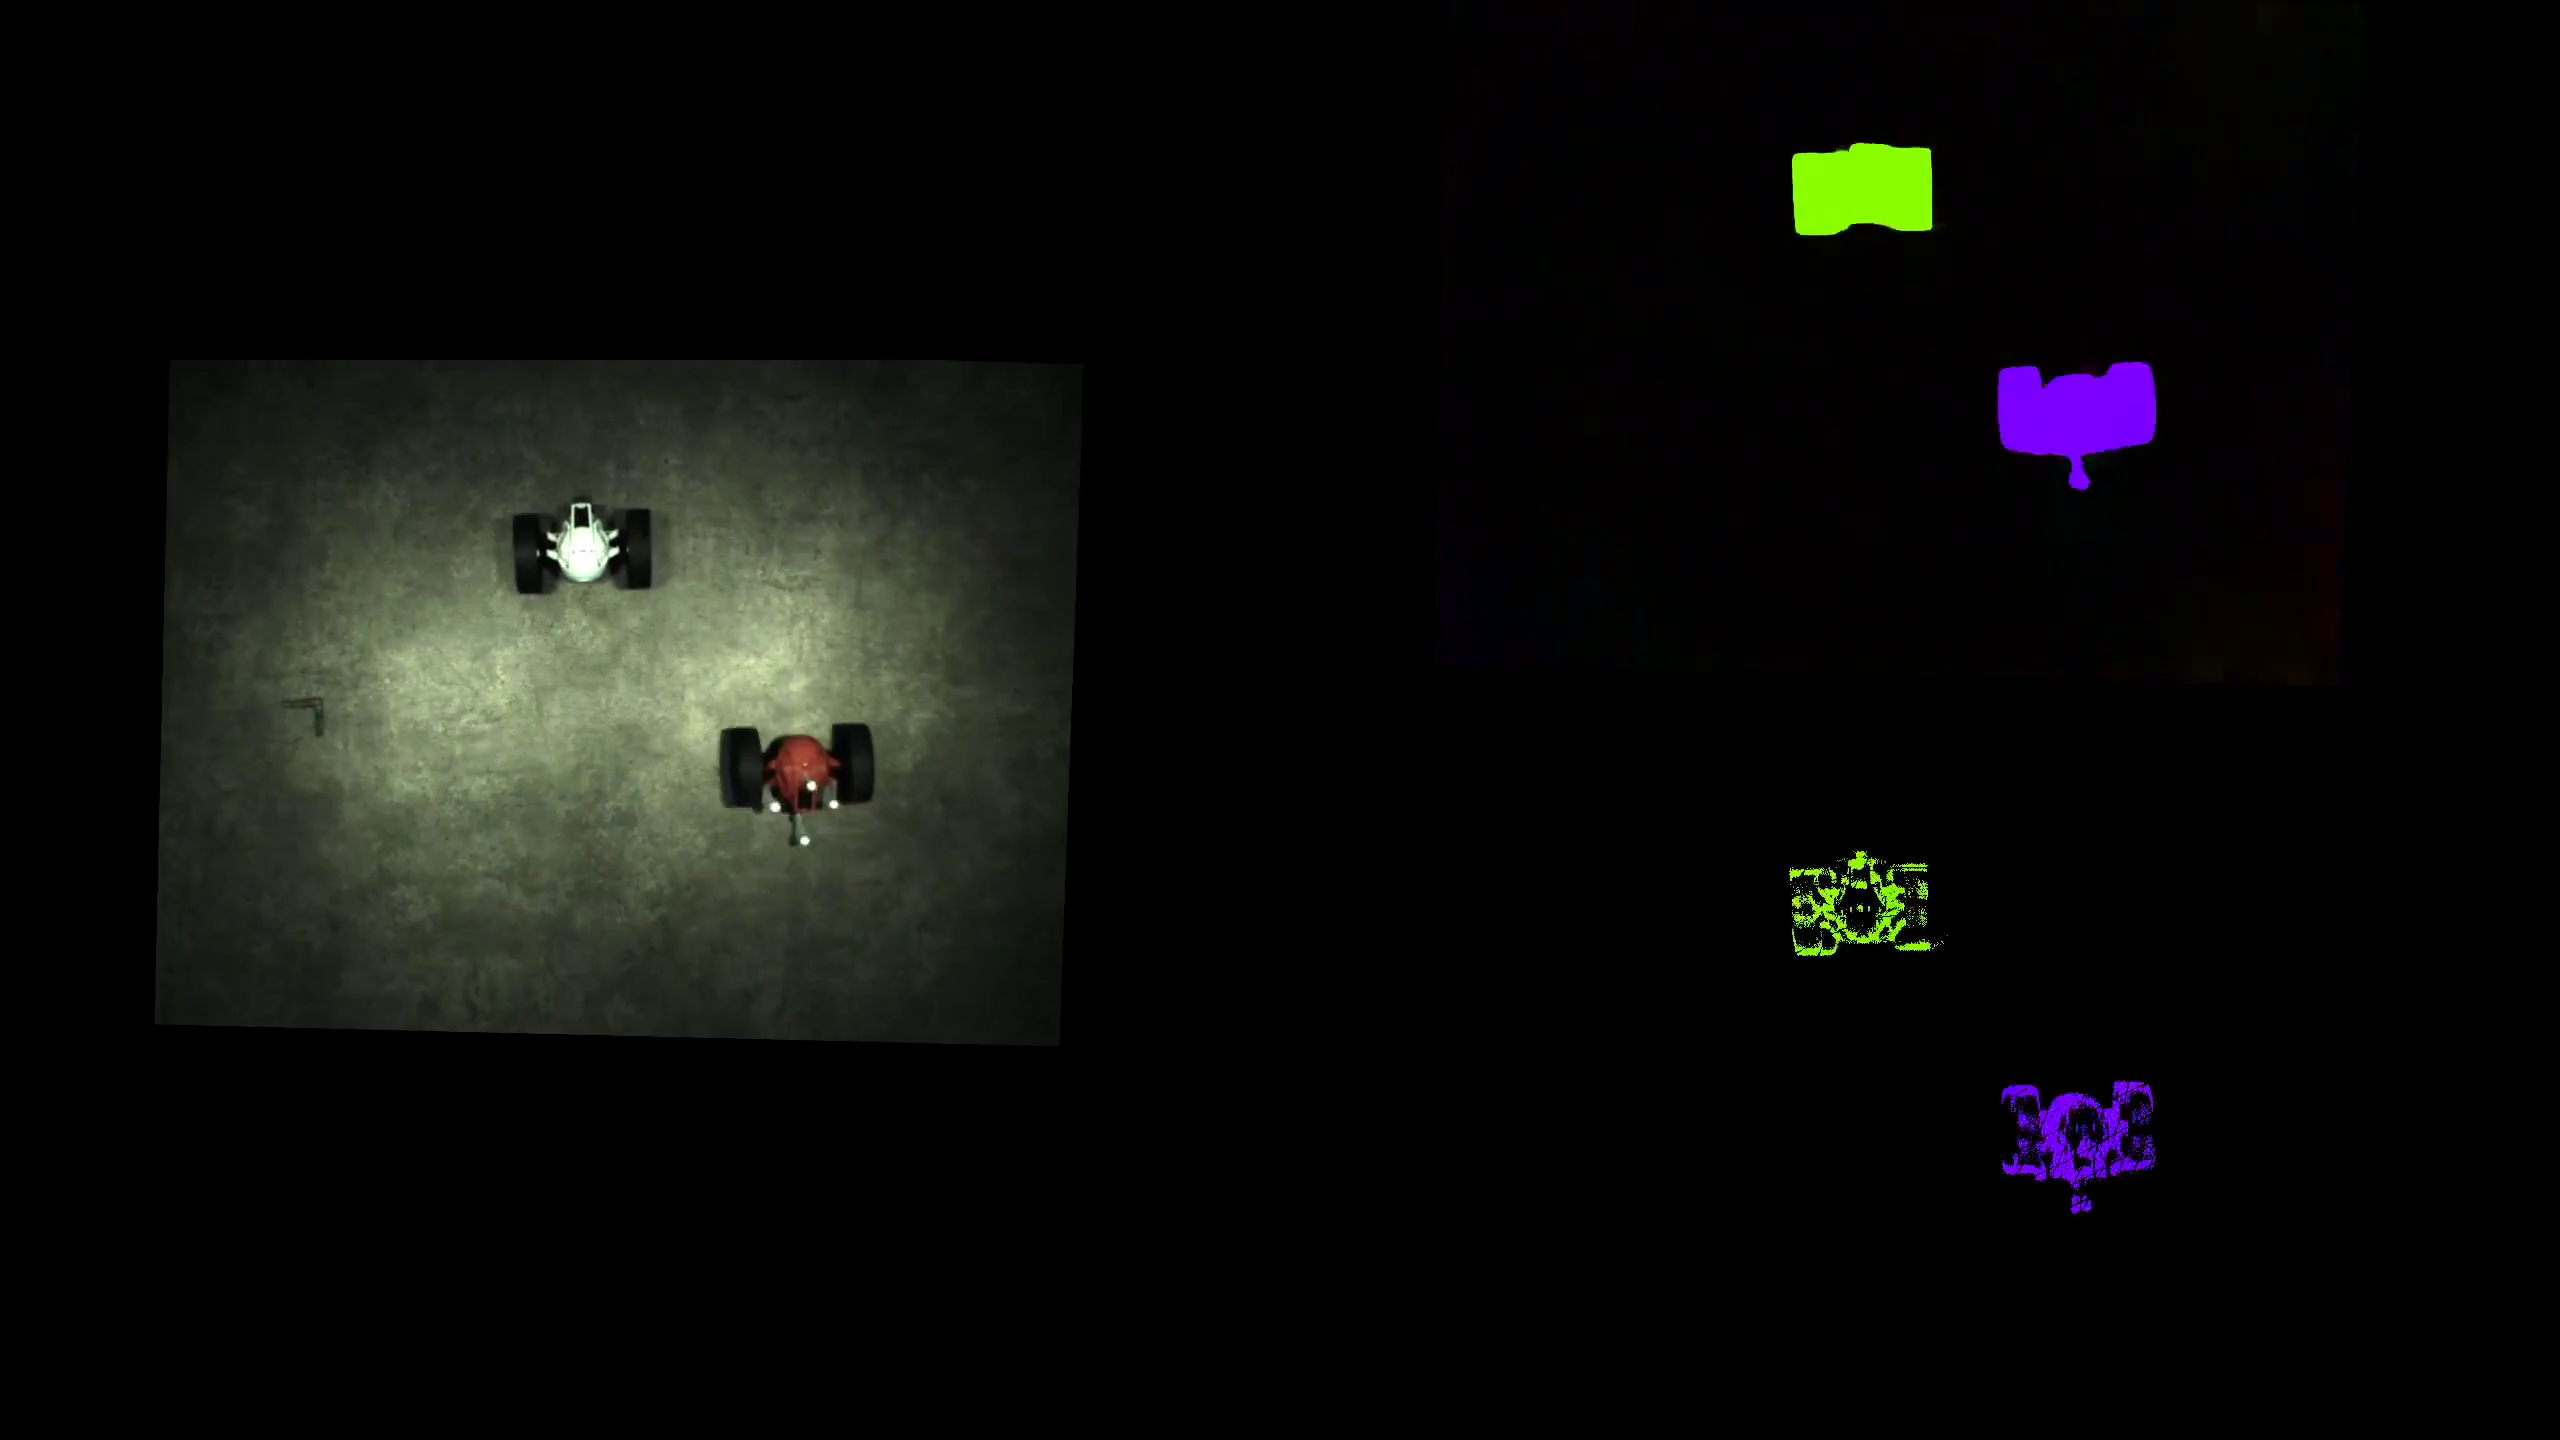
\includegraphics[width=0.85\linewidth]{mainmatter/figures/a_additional_exp/of_dataset/of_results.png}
  \caption{Example results on the dataset. Left is the view from the RGB camera (after applying the homography), top right is the frame-based optical flow from RAFT, and bottom right is our event-based optical flow.}\label{fig:appendix:add_exp:of_results}
\end{figure}

In the end, this dataset was not used as part of the evaluation of the final work, due to its simplicity and due to the \acrshort{fwl} metric allowing for an evaluation on any event-based dataset. Yet, it was a useful tool for initially designing, tweaking, and verifying the performances of our method on simple scenarios.

\subsection{For Depth Estimation}
As described in \cref{sec:conclusion:perspectives}, one of the parallel works of the thesis was conducted on the potential recording of a dataset using the robotized Renault Zoe cars of the lab, for depth estimation. Such a dataset was never actually recorded in the end, but we describe here the works conducted on calibration and synchronization.

\subsubsection{Calibration}
One of the first issues that we encountered while trying to record sequences was on the projection of LiDAR points into the frame of the event camera. Doing so required a calibration between the two sensors, an issue which had not been explored in details in the literature at the time (only a single method was available~\cite{Song2018CalibrationOE} but with moderate accuracy, more works on that topic have been published since~\cite{,Ta2022L2ELT,Jiao2023LCECalibAL}). Fortunately, the Hesai Pandora LiDAR that we used also contained five cameras as an all-in-one sensor, with all modalities being factory-calibrated both intrinsically and extrinsically. Therefore, our problem was simplified to a frame- to event-based calibration (while keeping in mind that this event-to-frames-to-LiDAR solution might be less precise than a direct LiDAR-to-event calibration).

However, this problem remains quite difficult: frame-based calibration often relies on a static pattern (e.g., a chessboard) being detected, but such a static pattern would not be visible for the event camera, making the calibration impossible. Also, for automotive applications, the focus of the camera is set further away than for more traditional indoor applications, meaning that a larger calibration board is required for its accurate detection. In order to solve these issues, we manufactured here a large, back-illuminated calibration board, with a ChArUco pattern on it. This calibration board is illustrated in \cref{fig:appendix:add_exp:depth_calib_board}.

\begin{figure}
  \centering
  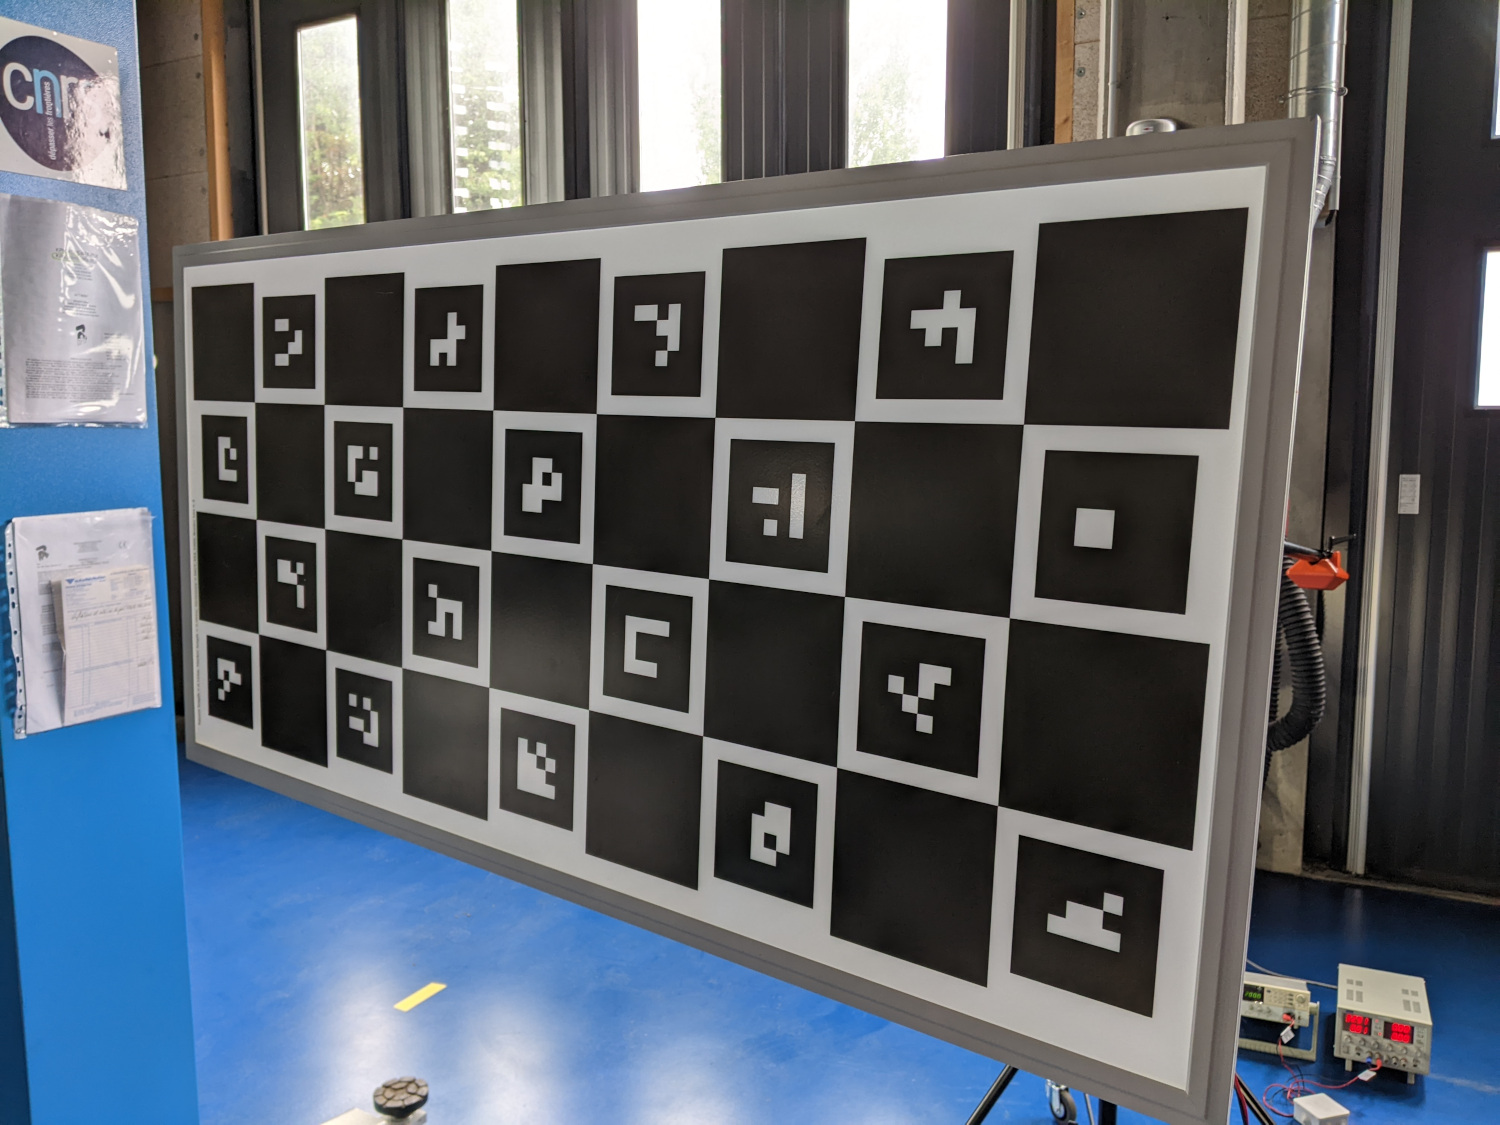
\includegraphics[width=0.49\linewidth]{mainmatter/figures/a_additional_exp/depth_dataset/board_close.jpg}
  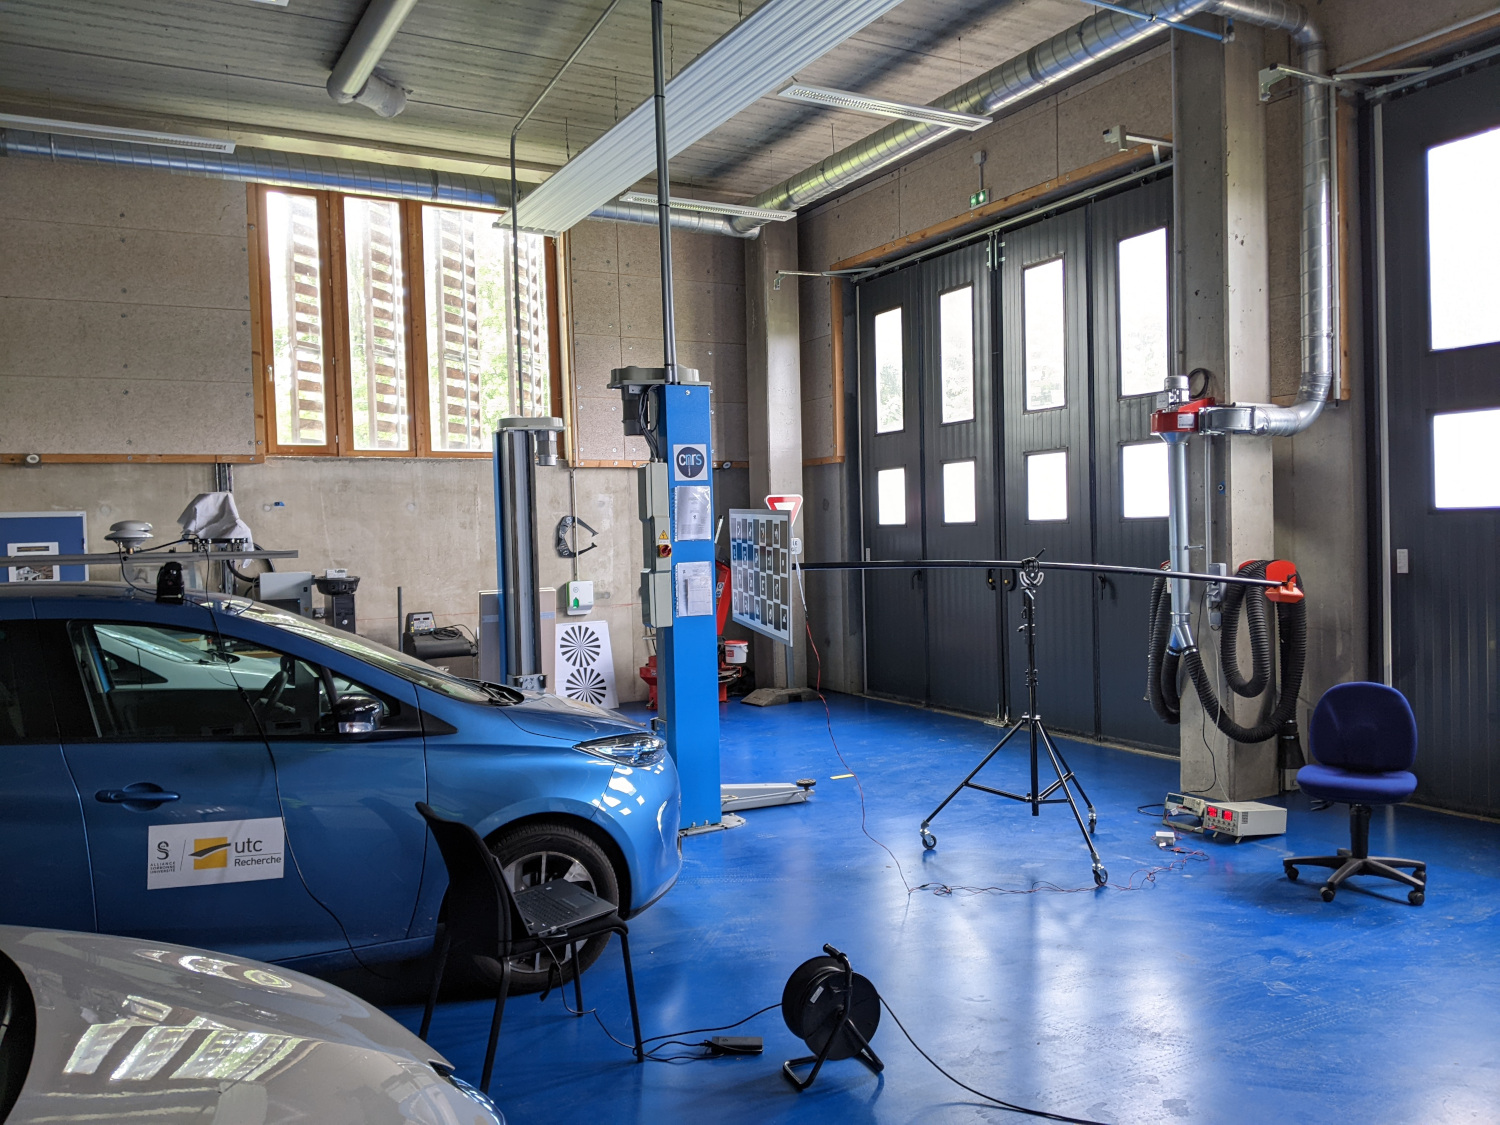
\includegraphics[width=0.49\linewidth]{mainmatter/figures/a_additional_exp/depth_dataset/board_large.jpg}
  \caption{Left: detailed view of the back-illuminated calibration board, with the ChArUco pattern. Right: larger view, showing the board positioned in front of the Zoe car, with the mechanical arm used for manipulating it.}\label{fig:appendix:add_exp:depth_calib_board}
\end{figure}

The main advantage of this setup is that, by making the back-light of the board blink at a high frequency, the event camera is able to detect this blinking for the white areas only, and therefore reconstruct an image of the board without any motion. As for the frame-based camera, this blinking is invisible due to its high frequency, and therefore does not disturb the board recognition. The choice of using a ChArUco pattern was also motivated by the fact that calibration can still be conducted even when the board is not fully visible for both cameras (which happened often in the configuration illustrated in \cref{fig:appendix:add_exp:depth_calib_board}) thanks to the unique tags, and by the ability of the Prophesee Gen4 camera to detect these tags perfectly thanks to its high-resolution.

Post-calibration results are shown in \cref{fig:appendix:add_exp:depth_superimposed}, where the event and LiDAR data appear to be adequately superimposed.

\begin{figure}
  \centering
  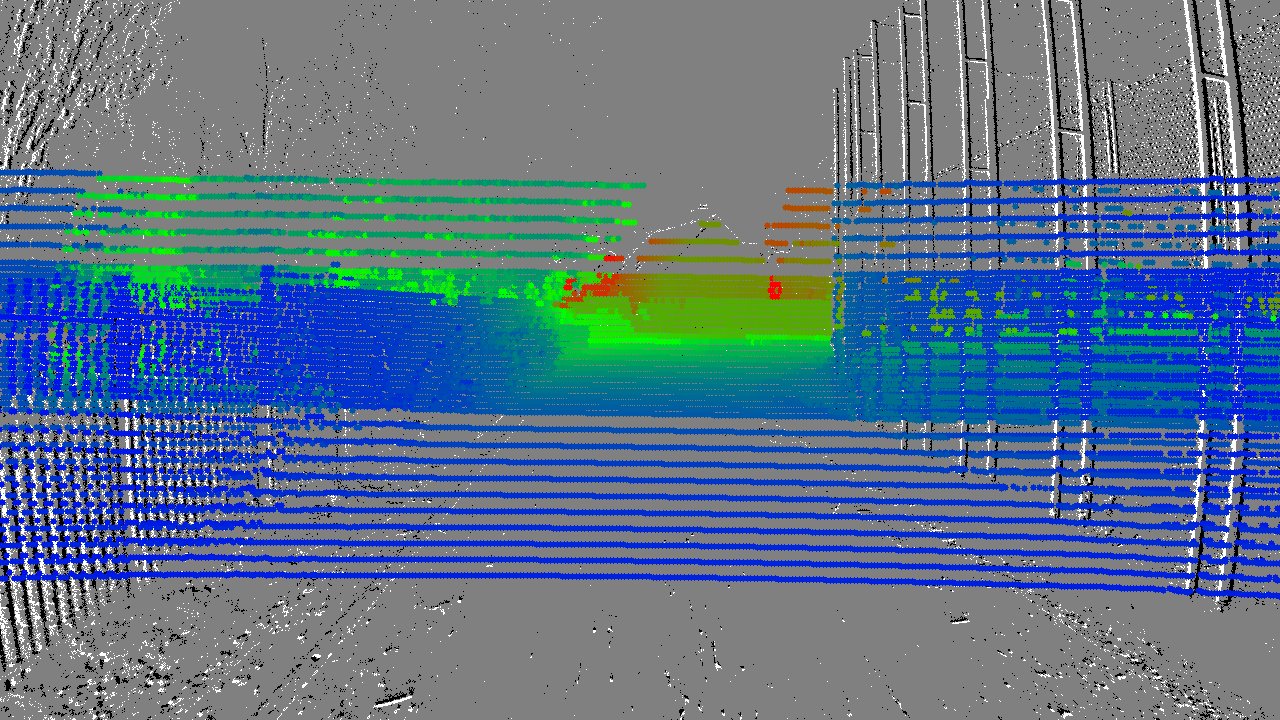
\includegraphics[width=0.49\linewidth]{mainmatter/figures/a_additional_exp/depth_dataset/evts_lidar_superimposed.png}
  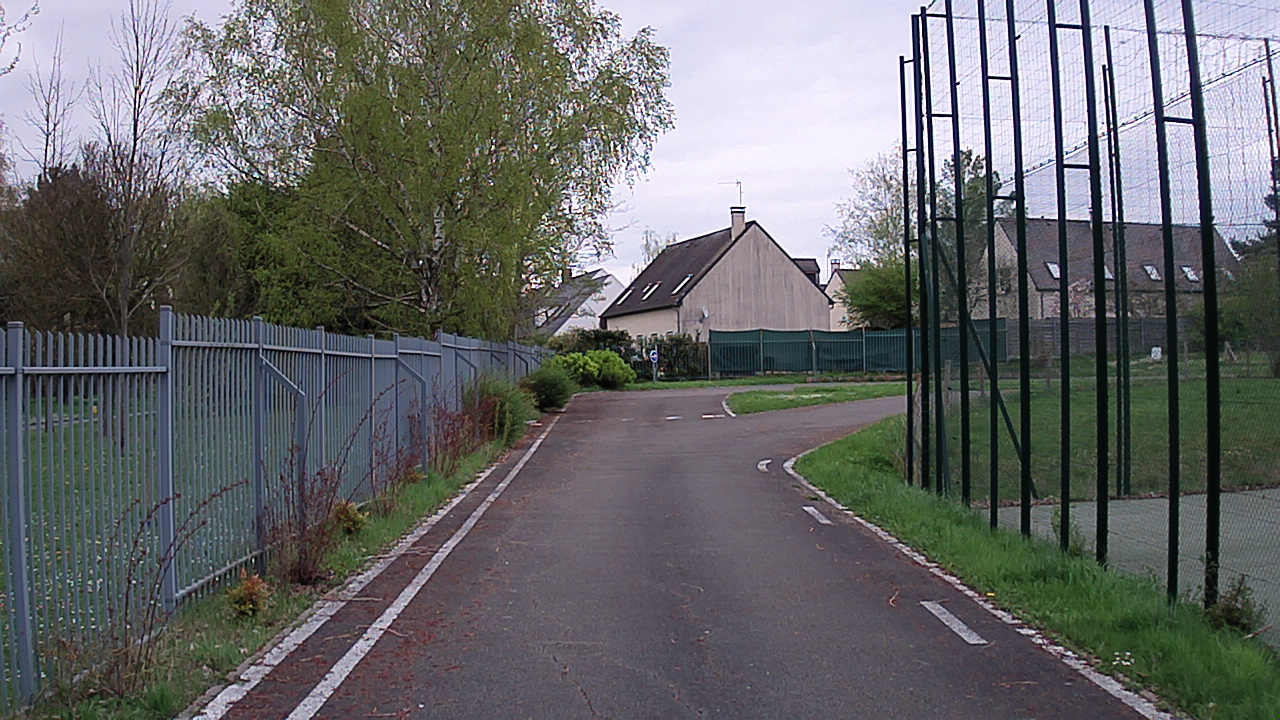
\includegraphics[width=0.49\linewidth]{mainmatter/figures/a_additional_exp/depth_dataset/rgb_ref.png}
  \caption{Left: superimposed event and LiDAR data following the calibration process. Right: reference RGB view of the scene, given for a better understanding.}\label{fig:appendix:add_exp:depth_superimposed}
\end{figure}

\subsubsection{Synchronization}
For the recording of the dataset, four main sensors were intended to be used. In addition to the Prophesee camera and the Pandora LiDAR described in the previous paragraphs, two high-speed RGB cameras were also planned to be used, for being able to construct dense stereo-based ground truth depth maps, as well as for making comparisons possible between event-based and frame-based methods on the same scenes. However, for both these purposes, an accurate synchronization of the sensors was necessary.

While the Pandora LiDAR and the RGB cameras were all \acrshort{ptp} (IEEE-1588) compatible, the Prophesee Gen4 camera transmits its data through USB, and can only be synchronized via external triggers. Therefore, as illustrated in \cref{fig:appendix:add_exp:sync}, while both the RGB and LiDAR sensors were synchronized through \acrshort{ptp}, the left RGB camera was physically connected to the Prophesee camera, and was configured to send a signal on this link every time a frame was captured. Upon reception, the Prophesee camera would mark this signal as a special ``trigger'' event, which could be easily identified. Following recording, a post-processing step was applied, to associate each trigger event to its corresponding image, and therefore its corresponding timestamp (as images are \acrshort{ptp}-timestamped). A simple interpolation was finally needed, to correct the timestamp of each individual event to its corresponding \acrshort{ptp} timestamp.

\begin{figure}
  \centering
  \begin{tikzpicture}[scale=0.75, every node/.style={transform shape}]
    % Changing the font
    \fontfamily{cmss}\selectfont

    % Nodes
    \node[draw, align=center, minimum size=3cm] (RGBl) {RGB camera\\(left)};
    \node[draw, align=center, minimum size=3cm, right= of RGBl] (E) {Prophesee\\camera};
    \node[draw, align=center, minimum size=3cm, right= of E] (L) {Pandora\\LiDAR};
    \node[draw, align=center, minimum size=3cm, right= of L] (RGBr) {RGB camera\\(right)};
    \node[draw, align=center, minimum size=3cm, below right=2cm and -1cm of E] (C) {Computer};

    % Links
    \draw[<->,>=latex, orange, line width=0.3mm] (C) -| (RGBl);
    \draw[<->,>=latex, blue, line width=0.3mm] (C) -- (E);
    \draw[<->,>=latex, orange, line width=0.3mm] (C) -- (L);
    \draw[<->,>=latex, orange, line width=0.3mm] (C) -| (RGBr);
    \draw[->,>=latex, gray, line width=0.3mm] (RGBl) -- ($(RGBl.north)+(0,1cm)$) -| (E);

    % Legend
    \node[minimum width=1cm, minimum height=0.75cm, below right=1cm and -1cm of C] (Eth) {};
    \node[minimum width=1cm, minimum height=0.75cm, below=0cm of Eth] (USB) {};
    \node[minimum width=1cm, minimum height=0.75cm, below=0cm of USB] (Phy) {};
    \draw[<->,>=latex, orange, line width=0.3mm] (Eth.west) -- (Eth.east);
    \draw[<->,>=latex, blue, line width=0.3mm] (USB.west) -- (USB.east);
    \draw[->,>=latex, gray, line width=0.3mm] (Phy.west) -- (Phy.east);
    \node[align=center, right=0.5cm of Eth] (Ethl) {Ethernet (data and PTP)};
    \node[align=center, right=0.5cm of USB] (USBl) {USB (data)};
    \node[align=center, right=0.5cm of Phy] (Phyl) {Physical link (triggers)};
  \end{tikzpicture}
  \caption{The synchronization system between the four sensors and the computer (which collects data and acts as the \acrshort{ptp} master).}\label{fig:appendix:add_exp:sync}
\end{figure}

The main issue of this method is that, in case of missing data (images or trigger events not being recorded), discrepancies in the timestamps would have been introduced, making the synchronization incorrect. During the tests we conducted, this case was often observed, with the recording containing a few more trigger events than images. However, a finer analysis showed that the additional triggers were always located at the very end of the sequence, and were in reality due to the RGB camera continuing to capture a few frames after being told to stop recording (and thus sending trigger signals), but not actually transmitting these frames.


\section{Extensions to the SLED Dataset}

\subsection{Ground Truth for Instance Segmentation}
During our tests for making the sparse attention-based depth estimation networks work in \cref{sec:delta}, we tried among other ideas to add a supervision loss on attention values (as described in \cref{sec:delta:sparse_network:issues:loss_att}). The idea here was that, if we would be able to force the network to put in relation events and LiDAR points belonging to the same object, then it would learn how to group them, and produce better depth estimations (especially for the sky, which was never recognized as being a special entity).

For that purpose, we tried adding a ground truth instance segmentation to the \acrshort{sled} dataset, for being able to identify independent objects, and therefore regroup events and LiDAR points correctly for the supervision loss. However, as shown in \cref{fig:appendix:carla:segmentation}, the instance segmentation maps in CARLA suffer from several issues (invisible objects, lack of precision for dynamic objects), and therefore they could not be used as part of this work.

\begin{figure}
  \centering
  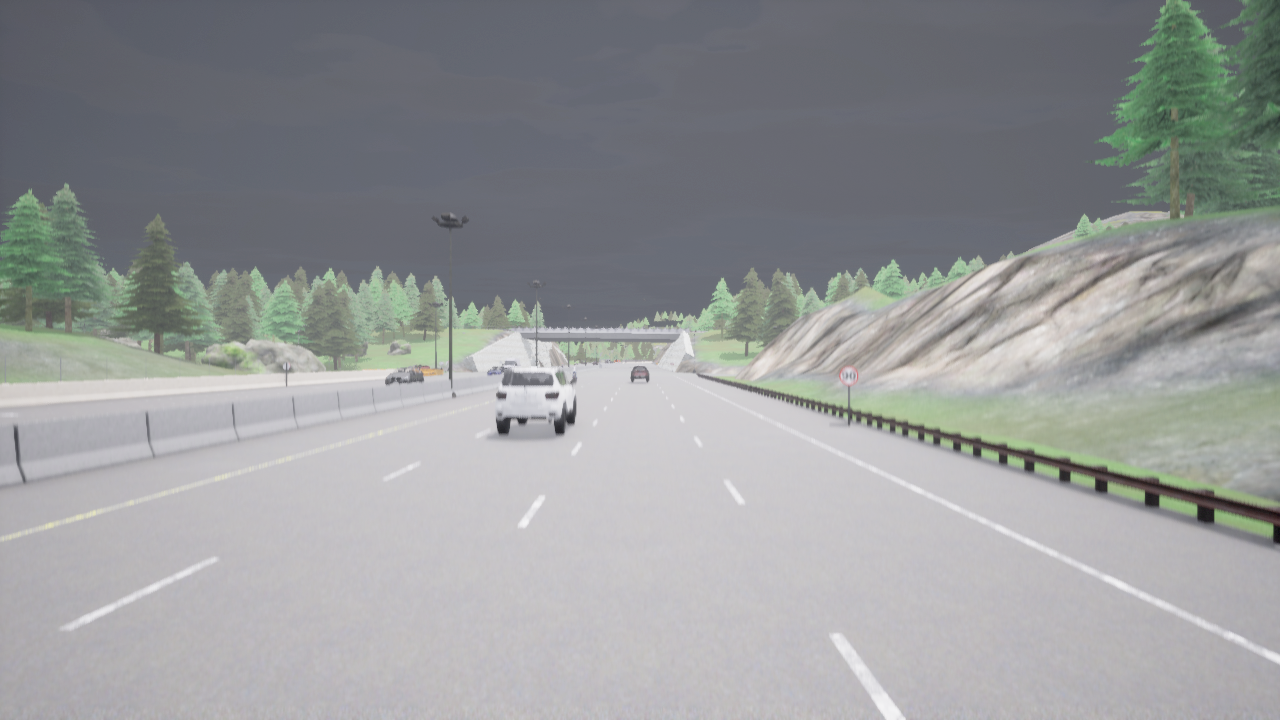
\includegraphics[width=0.9\linewidth]{mainmatter/figures/a_additional_exp/carla/segmentation_rgb.png}
  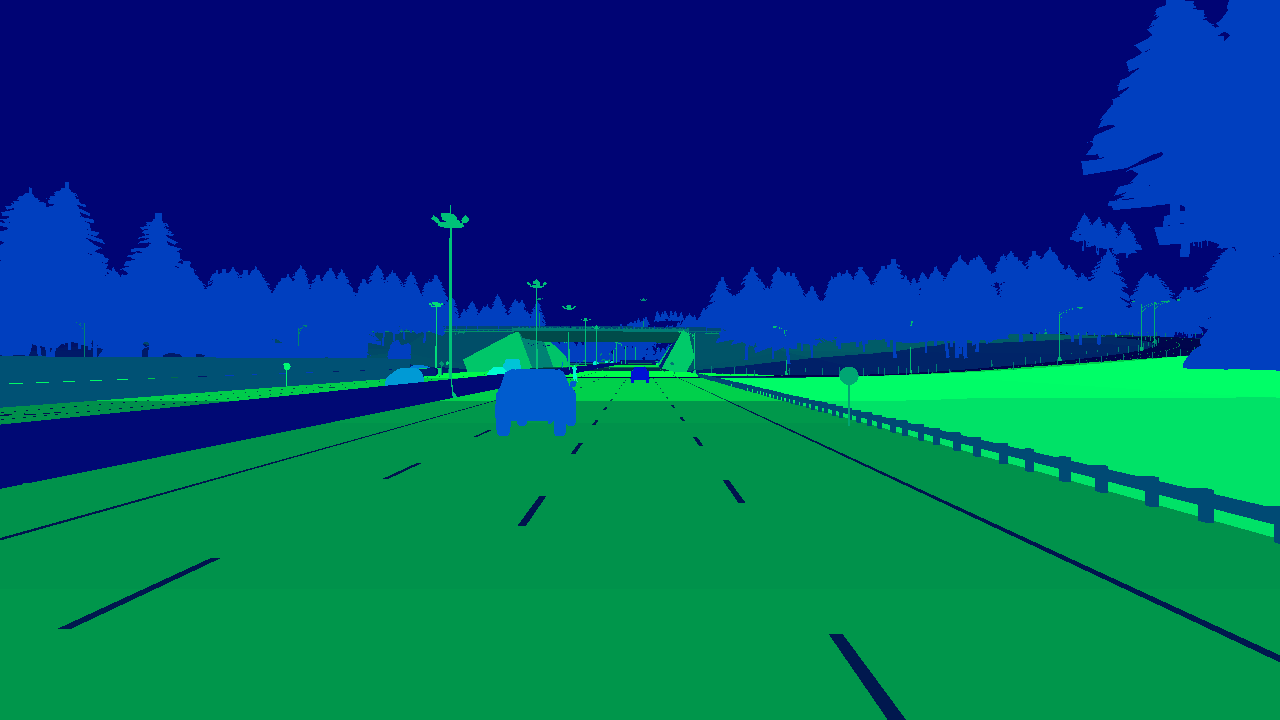
\includegraphics[width=0.9\linewidth]{mainmatter/figures/a_additional_exp/carla/segmentation_map.png}
  \caption{Illustration of the segmentation issue in CARLA. Top: RGB view of the scene. Bottom: corresponding segmentation map; note how the hills on the left and right extremities are missing in this segmentation map, making objects behind them appear, and how rough the segmentation is for the leaves of the trees.}\label{fig:appendix:carla:segmentation}
\end{figure}

As an alternative, we tried computing instance segmentation by using external tools like the Segment Anything method from Meta~\cite{Kirillov2023SegmentA} on the RGB images of the dataset, but this approach yielded suboptimal results, due to a lack of temporal stability of the segmented areas, and due to a lack of precision at the edges of the objects.

\subsection{Additional Maps}
As noted in \cref{sec:aled} (\cref{tab:aled:sled_content}), our \acrshort{sled} dataset was built from data collected in the \verb|Town01| to \verb|Town07| and \verb|Town10| maps of CARLA (\verb|Town08| and \verb|Town09| being unseen maps used as part of the evaluation of CARLA's autonomous driving leaderboard\footnote{\url{https://leaderboard.carla.org}}). However, following the initial publication of our dataset, several maps have been added to CARLA, namely, \verb|Town12| (in beta in version 0.9.14, and officially released in version 0.9.15), and \verb|Town13 and \verb|Town15 (in beta in version 0.9.15). These three maps (and especially \verb|Town12| and \verb|Town13|) offer new, large environments, with some novel unique features, as illustrated in \cref{fig:appendix:carla:town12}. Being able to integrate them in \acrshort{sled} would allow for a more complete and a more diverse dataset, and could allow for a better training and evaluation.

\begin{figure}
  \centering
  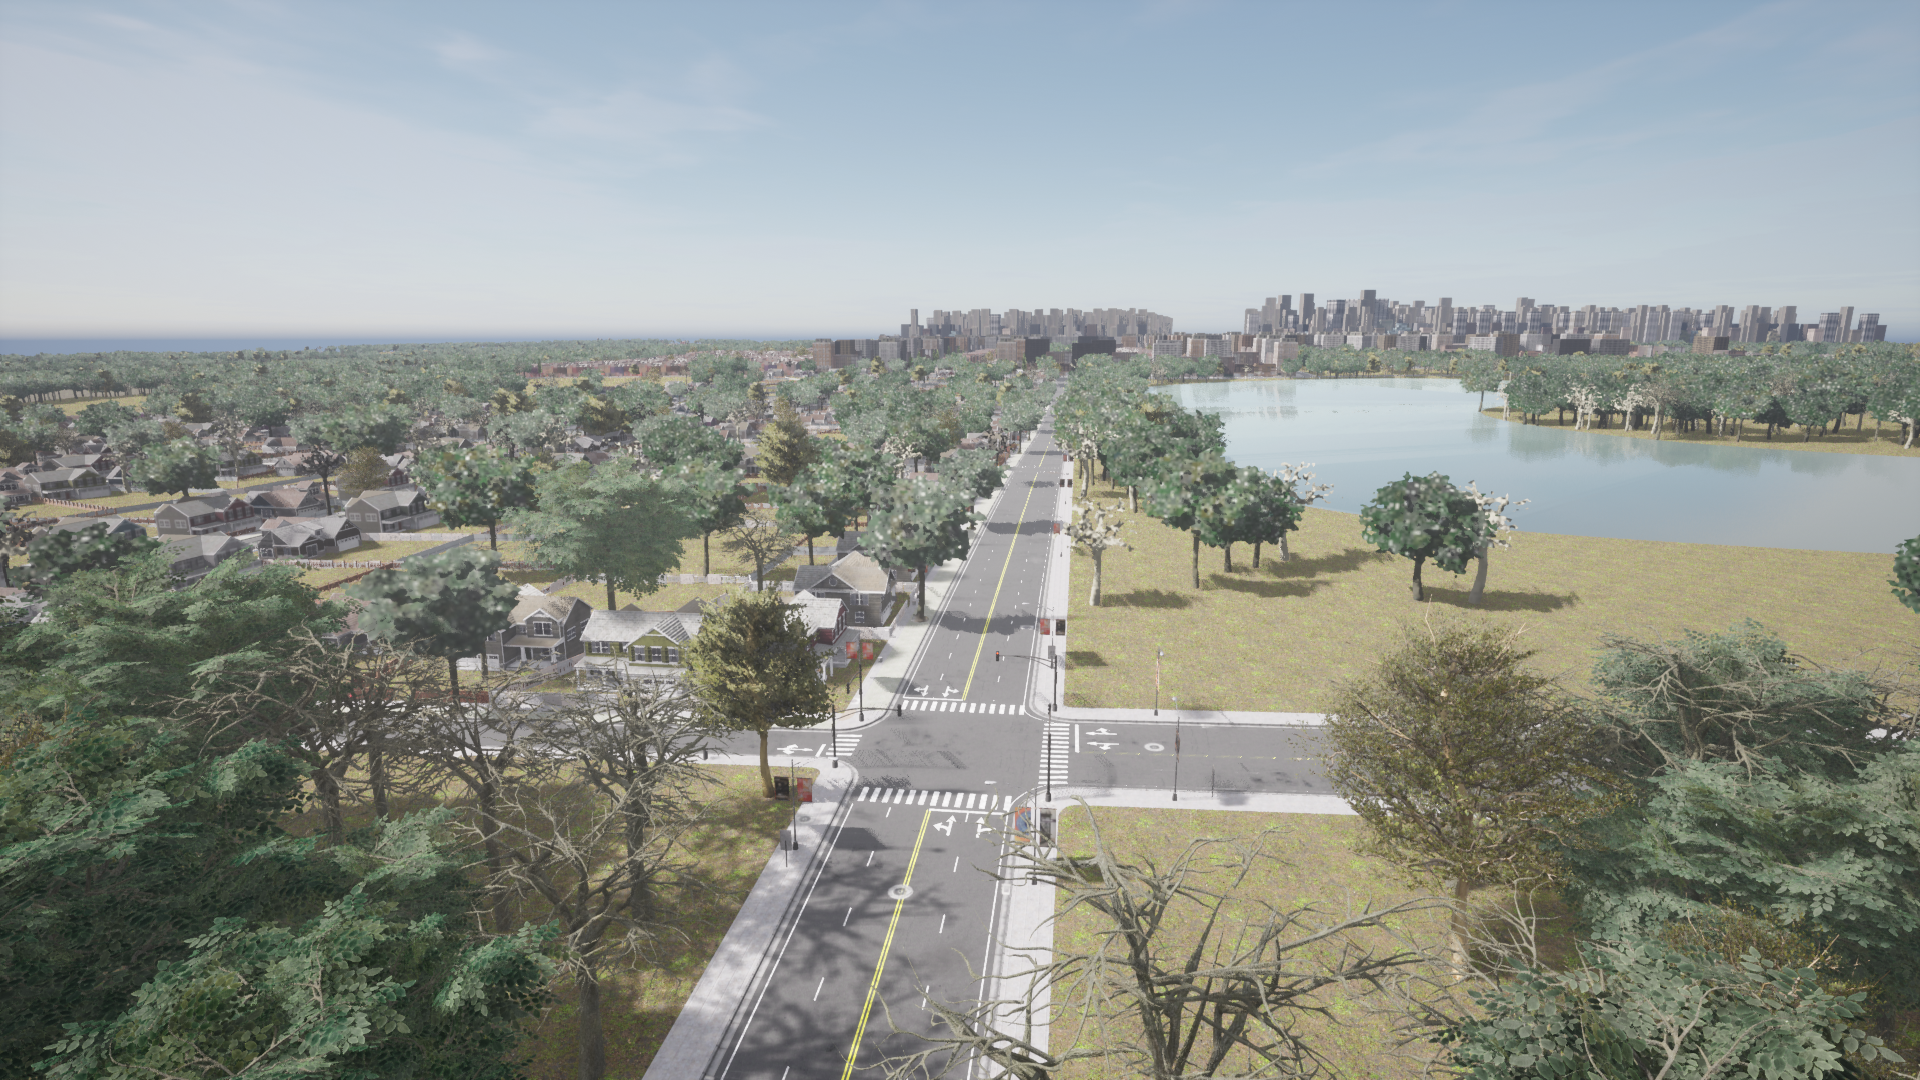
\includegraphics[width=0.9\linewidth]{mainmatter/figures/a_additional_exp/carla/town12.png}
  \cprotect\caption{Overview of the \verb|Town12| map. A residential area can be seen on the left, a large body of water on the right, and buildings can be seen at the back.}\label{fig:appendix:carla:town12}
\end{figure}

However, as of the writing of this thesis, these maps still suffer from technical issues, and have not been integrated in \acrshort{sled} yet. One such issue, for instance, is the inability to have any pedestrian in \verb|Town12|, as no spawn location has been provided for them (\url{https://github.com/carla-simulator/carla/issues/6552}). Therefore, like for the instance segmentation, we are waiting for fixes to these issues to be published, in order to upgrade the dataset in the future.
